%%%%%%%%%%%%%%%%%%%%%%%%%%%%%%%%%%%%%%%%%%%%%%%%%%%%%%%%%%%%%%%%%%%%
%%%%%%%%%%%%%%%%%%%%%%%%%%%%%%%%%%%%%%%%%%%%%%%%%%%%%%%%%%%%%%%%%%%%
\definecolor{charcoal}{gray}{0.30}
\lstdefinestyle{console}
{language=bash,
basicstyle=\scriptsize\ttfamily\color{white}\bfseries,
backgroundcolor=\color{charcoal},
keywordstyle=\color{white},
alsoletter={:~\$},
}

\chapter{Installation}

% ==================================================================
\section{Overview}

\begin{figure}[!h]
	\centering
	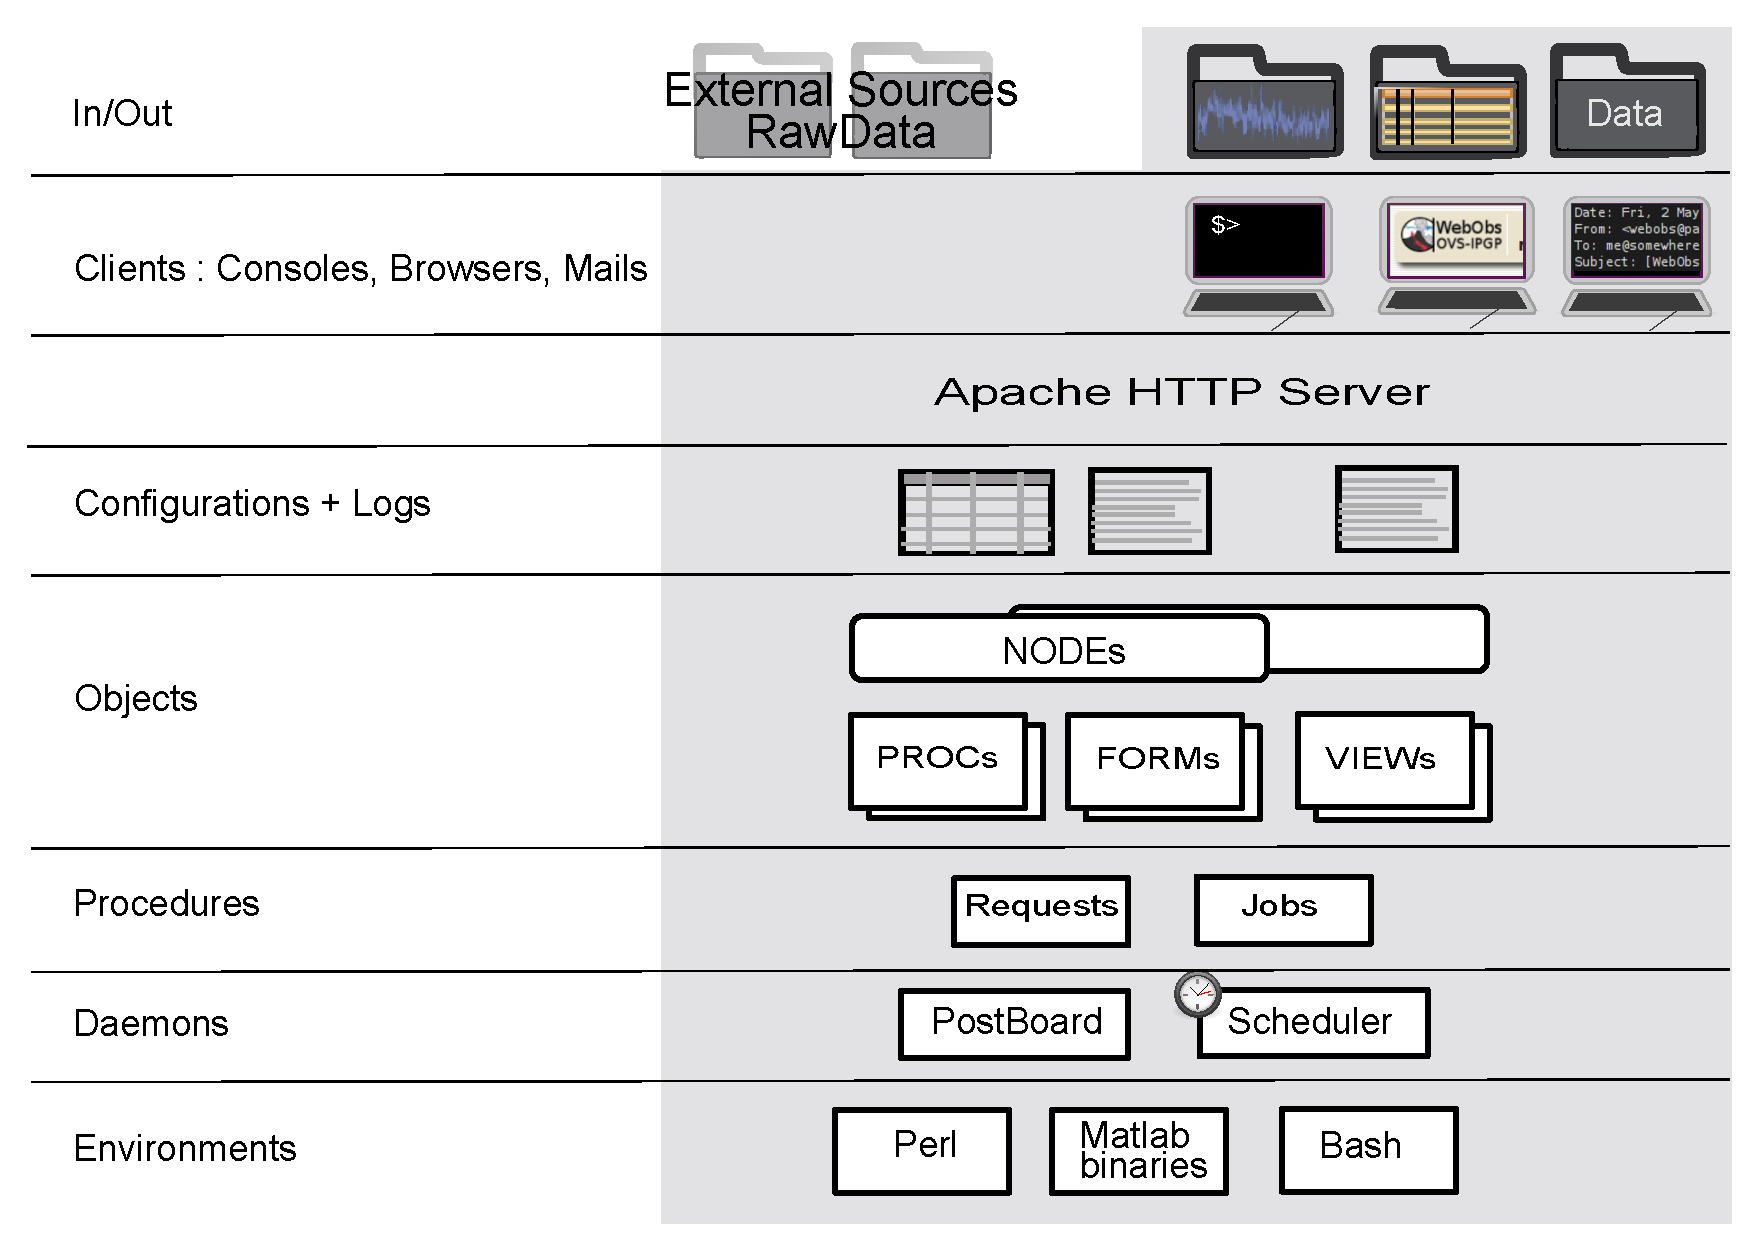
\includegraphics[width=\textwidth]{figures/bigwo.pdf}
	\caption{\webobs big picture}
\end{figure}

% ==================================================================
\section{System requirements}

\subsection{System and package}

\webobs server can run on \textbf{Linux} and \textbf{Mac OS X}.

It has been successfully installed/tested on:
\begin{itemize}
\item   Linux 3.13.0 , x86\_64 , Ubuntu 14.04 LTS
\item   Linux 4.13.0 , x86\_64 , Ubuntu 16.04 LTS
\item   Linux 2.6.32, i386 , Debian 2.6.32-48squeeze4
\item   Linux version 3.2.0-4-amd64, Debian 3.2.51-1
\item   Linux version 3.2.0-4-amd64, Debian 4.6.3-14
\item   Linux version 4.9.0-5-amd64, Debian 4.9.65-3
\item   Mac OS X 10.11.5, Darwin 15.5.0
\end{itemize}

\webobs (browser) clients have been successfully tested with:
\begin{itemize}
\item   FireFox (up to FireFox 47)
\item   Safari
\end{itemize}

\fbox{
	\parbox{\textwidth}{
	Download  the \webobs latest Release and \textbf{MatLab} Runtime Compiler from:\\
	\textbf{http://www.ipgp.fr/\textasciitilde beaudu/webobs.html}
	}
}

% -----------------------------------------------------------------
\subsection{Software requirements}

\subsubsection{Required installations}

The following softwares will be tested for existence by the \textbf{setup} installation procedure:

\begin{itemize}
\item   Perl 5.14+ (\textbf{setup} will also check for additional Perl modules)
\item   Apache 2.2+
\item   Sqlite 3.7.9
\item   ImageMagick 6.6.9 (convert+identify)
\item   Mutt 1.5+
\item   MatLab MCR R2011b
\end{itemize}

\subsubsection{Bundled software}

The following lists softwares included in \webobs package:

\begin{itemize}
\item   SeisComP3 (slinktool + arclink\_fetch)
\item   JavaScript extensions:
\begin{itemize}
\item   JQuery
\item   flot
\item   markItUp
\item	MultiMarkDown
\item   overlib
\end{itemize}
\end{itemize}

% ==================================================================
\section{Initial installation}

You must have \textbf{root} privileges to execute \webobs installation. 

\textbf{Installation procedure}:

\begin{itemize}
\item   Choose/create your target \webobs directory, and \wocmd{cd} to it. For
demonstration purposes in this document we will use \wocmd{/opt/webobs/} as the target \webobs directory. 
\item   Download \webobs package and \textbf{MatLab RunTime Compiler}. For
demonstration purposes in this document we will use \wocmd{WebObs-\release.tgz} as the \webobs package. 
\item   Choose/create the system's \webobs user+group (aka \wocmd{WebObs Owner}) if you don't want \wocmd{setup} procedure
to create one itself.

\fbox{
	\parbox{\textwidth}{
	The \webobs \textbf{user}, and its corresponding \textbf{group}, is the required \webobs administration account. 
	It must have a home directory. It will be the owner of the \webobs CONF,LOGS,DATA,WWW,OUTx directories.  
	The Apache http server user will be made a member of \webobs user's group.
	The \webobs user can be used to launch the \webobs Scheduler and Postboard daemons.
	}
}

\item   Untar \webobs package. This will create/populate the \webobs version subdirectory: 
\wocmd{/opt/webobs/WebObs-\release}.
\item   Run the \wocmd{setup} procedure (again, with \wocmd{root} privileges):
\begin{itemize}
\item   must be called as \wocmd{/opt/webobs/WebObs-\release/SETUP/setup}
\item   \wocmd{setup} will gather information/location from your system/environment,
check for some dependencies (see Requirements section above), build the \webobs
structure, optionaly customize Apache's \webobs Virtual Host, set required system's
ownerships and access-rights, and populate your brand new \webobs with 
ready to use demonstration data and templates.
\item   once completed, \wocmd{setup} will display \webobs configuration (see \wocmd{qsys} command below).
\item   \webobs now ready, you need to activate the \wocmd{scheduler}, \wocmd{postboard} and (re)start Apache http server. 
\end{itemize}
\end{itemize}

\begin{figure}[!h]
	\centering
	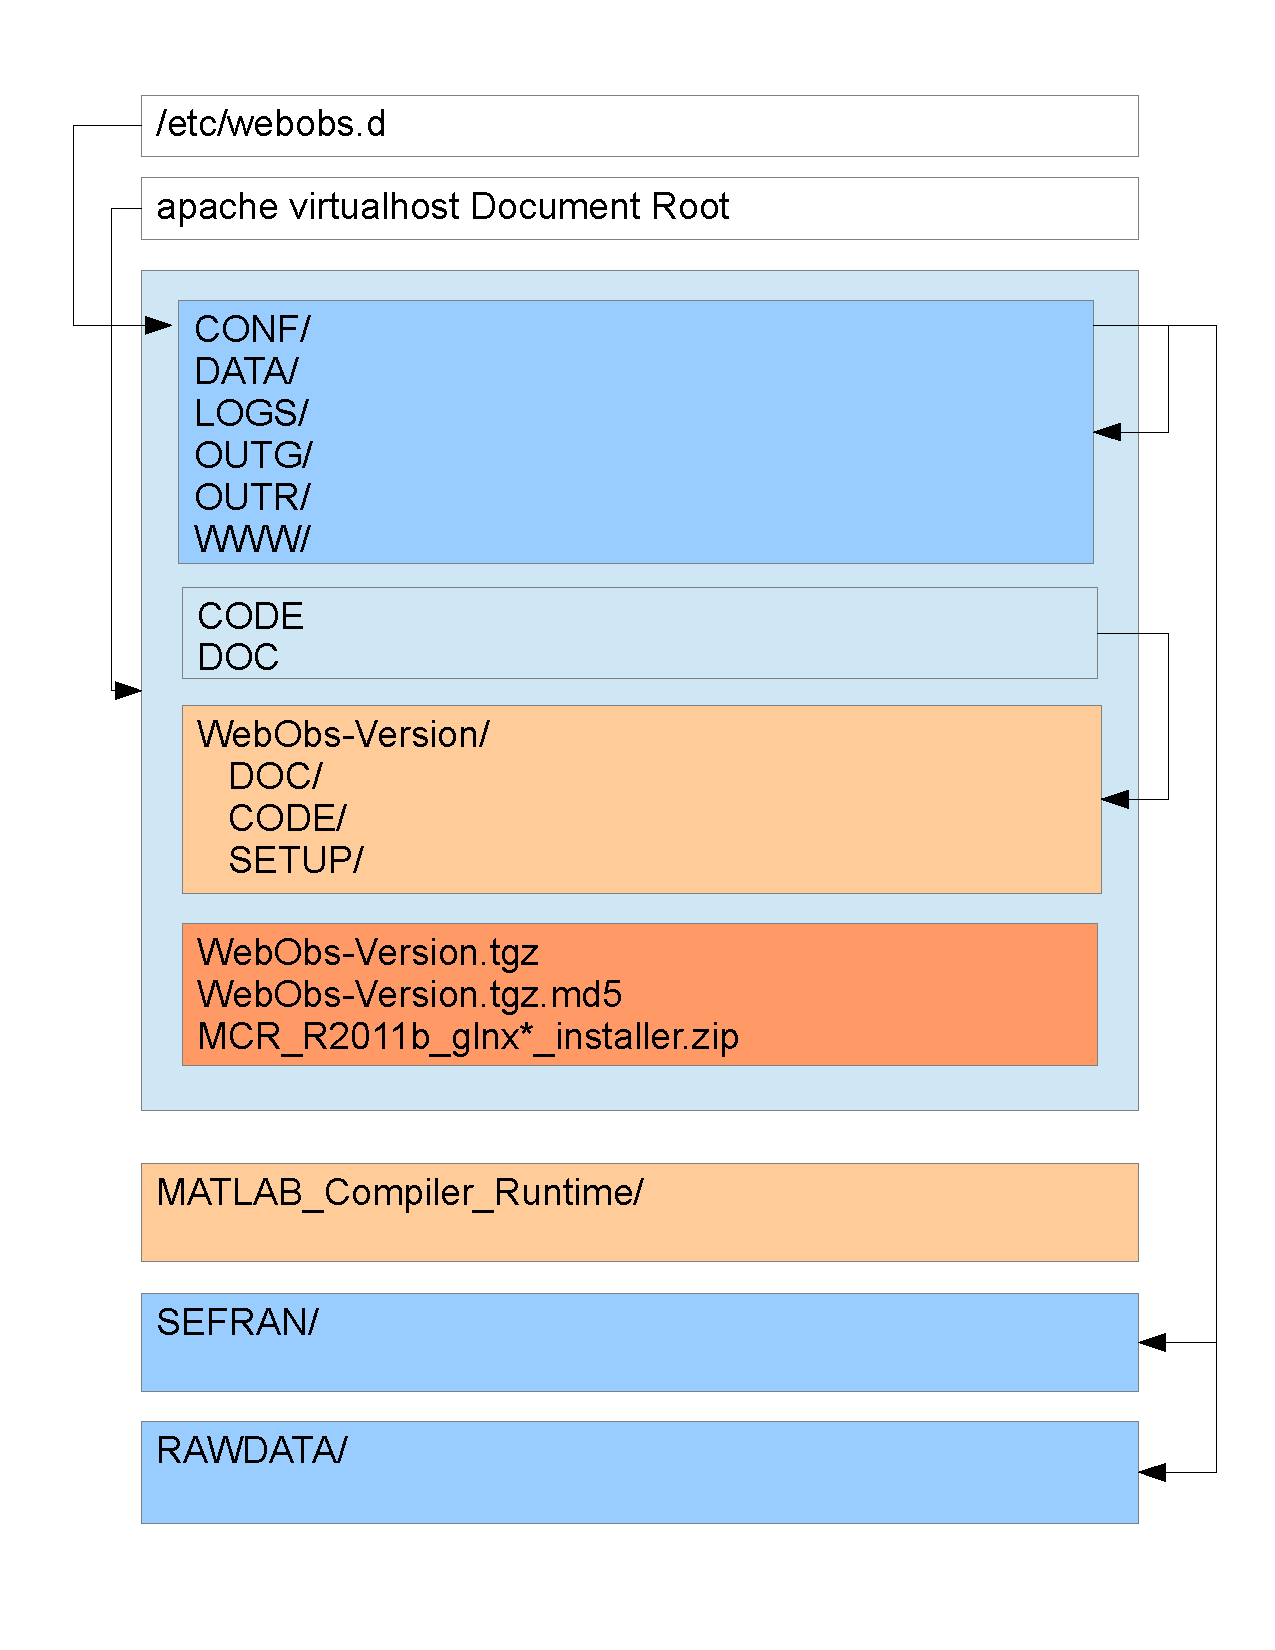
\includegraphics[width=\textwidth]{figures/disk_overview.pdf}
	\caption{Overview of \webobs installed disk structure}
\end{figure}

% ==================================================================
\section{Upgrades}

You must have \textbf{root} privileges to execute \webobs upgrades.

The \wocmd{setup} procedure used for Initial Installation, is also used to upgrade \webobs to a new release.
It will automatically detect that an upgrade is intended rather than a first time installation.

\textbf{Upgrade procedure:}

\begin{itemize}
\item   Download \webobs package corresponding to the version you want to upgrade to.
\item   Untar \webobs package.
\item   Run the \wocmd{setup} procedure (\wocmd{/opt/webobs/WebObs-\release/SETUP/setup}).
\item   \wocmd{setup} reports Version changes and important information in the
\wocmd{SETUP.CONF.README} file. Please read it carefully.
\item   \wocmd{setup} will also, if you choose to do so, walk through executions of 
\wocmd{vimdiff}s between your configuration files and corresponding 
non-customized \webobs version
configurations that were changed / added. 
\end{itemize}

% ==================================================================
\section{qsys - query configuration}

\wocmd{qsys} script, also automatically executed when \wocmd{setup} ends, will
display your base \webobs configuration.

\begin{lstlisting}[style=console,title=\wofile{qsys} example]
                                     __ __ __
             ...oooooWoooooo..     W \ V  V /          Id: ipgp
          .oo.. ............o..o.. W  \_/\_/      Version: WebObs-beta-1.8.2
       .oo.     ..............  ..oW   ___ 
     .oo.      ...............     W  / -_)         Owner: webobs[webobs]
    .W..     .  .............o.... W  \___|          Root: /opt/webobs
   .W.............o.........oWWWoo.W   _           Config: /opt/webobs/CONF/WEBOBS.rc
  .W    .   .  . ............o.....W  | |__          Logs: /opt/webobs/LOGS
  W.        ..   .WWWWo....  .     W  | '_ \
 .W        .Wo. .Wxxxxx....        W  |_.__/          MCR: /usr/local/MATLAB/MATLAB_Compiler_Runtime/v7...
 .W        .WWW.WxxxxxxW...   ...  W   ___        Rawdata: /opt/rawdata
 .W       .WWWWWxxxxxxxxW..........W  / _ \        Sefran: /opt/sefran
  Wo..ooWxxxxxxWxxxxxxxxxxo........W  \___/
  .xxxxxxxxxxxxxxWxxxxxxxxxW.......W   _             HTTP: http://webobs.ipgp
   .xxxxxxxxxxxxxWWWWWxxxxxxW.....oW  | |__                /etc/apache2/sites-available/webobs
    .WxxxxxxxxxWxxWWWWWWWxxxxxWWo..W  | '_ \               running on Apache/2.2.22 (Ubuntu)
     .oxxxxxxxxxxxxxWWWWWWWxxxxxxxWW  |_.__/
       .oWxxxxxxxxxxxxxWWWWWWWWxxxWW   ___      Scheduler: not running
          .oWxxxxxxxxxxxxWWWWWxW.. W  (_-<      PostBoard: not running
             ...oWWWxxxWWWWo..     W  /__/
                                                                qsys run 2014-08-08 12:05:06

\end{lstlisting}

% ==================================================================
\section{Configuration files syntax}

\webobs configuration files (*.rc, *.conf, or *.cnf) used to customize your installation
and described in this document, typically define one 
functionnal parameter (\wocmd{key}) per line, made up of one or more associated values
(\wocmd{fields}). They can share the same set set of syntactic rules for  
parsing/interpretation:

1) In order to be parsed/interpreted according to the following rules, the files must
contain a so-called 'definition line' (identified with \wocmd{=} in column 1) as the 
first interpreted line. This definition line is also used to further define parsing, 
that comes in two (2) flavors:

\begin{tabular}{ll}
\wocmd{=key\textbar value}  &  one value per key (Perl's equiv. \$X\{key\} =\textgreater value)\\
\wocmd{=key\textbar name1\textbar ...\textbar nameN}  & multiple named values per key (Perl's equiv. \$X\{key\}\{name1\} =\textgreater value)\\
\end{tabular}

2) Any text following a \wocmd{\#} is considered a comment and discarded.

3) Blank lines are discarded, leading and trailing blanks too.

4) Fields separator character, within interpreted lines, is \textbar (pipe).

5) \wocmd{\textbar} and \wocmd{\#} characters that must belong to a field value may be 
'escaped' (ie. not interpreted as separator or comment respectively) by prefixing them 
with a \textbackslash .

6) Field value substitution (interpolation) is allowed in \wocmd{=key\textbar value} format:

\begin{tabular}{ll}
\wocmd{\$\{key\} in value}       & will be replaced with the value of the key \textbar value pair of the current file.\\
\wocmd{\$WEBOBS\{key\} in value} & will be replaced with the value of the \webobs main configuration \wocmd{key} value. \\
\end{tabular}


% ==================================================================
\section{\webobs tree}
%\begin{table}[p]
\begin{center}
    \begin{longtable}{ll}
		\fcolorbox[gray]{0.1}{0.9}{\wocmd{CONF/}} & configurations  \\
	    \hspace{0.4cm} \wocmd{WEBOBS.rc}             & main \webobs configuration file  \\
	    \hspace{0.4cm} \wocmd{*.\{rc,conf,cnf\}}     & other configuration files \\
	    \hspace{0.4cm} \wocmd{FORMS/}                & FORMS definitions \\
	    \hspace{0.8cm} \wocmd{formname/}             & definitions for FORM formname    \\
	    \hspace{0.4cm} \wocmd{PROCS/}                & PROCS definitions \\
	    \hspace{0.8cm} \wocmd{procname/}             & definitions for PROC procname    \\
	    \hspace{0.4cm} \wocmd{VIEWS/}                & VIEWS definitions \\
	    \hspace{0.8cm} \wocmd{viewname/}             & definitions for VIEW viewname    \\
	    \hspace{0.4cm} \wocmd{GRIDS2FORMS/}          & links from PROCs to FORMS  \\
	    \hspace{0.8cm} \wocmd{PROC.pname.formname}   & -\textgreater ../formname  \\
	    \hspace{0.4cm} \wocmd{GRIDS2NODES/}          & links from GRIDs to NODES  \\
	    \hspace{0.8cm} \wocmd{PROC.pname.nodename}   & -\textgreater ../../DATA/NODES/nodename  \\
	    \hspace{0.8cm} \wocmd{VIEW.vname.nodename}   & -\textgreater ../../DATA/NODES/nodename  \\
	    \\
		\fcolorbox[gray]{0.1}{0.9}{\wocmd{CODE/}} & \webobs code  \\
	    \hspace{0.4cm} \wocmd{bin/}                  & executables                \\
	    \hspace{0.4cm} \wocmd{cgi-bin/}              & Perl CGIs                  \\
	    \hspace{0.4cm} \wocmd{css/}                  & HTML Style Sheets          \\
	    \hspace{0.4cm} \wocmd{html/}                 & static HTML pages          \\
	    \hspace{0.4cm} \wocmd{icons/}                & HTML icons, static images  \\
	    \hspace{0.4cm} \wocmd{js/}                   & javascript                 \\
	    \hspace{0.4cm} \wocmd{matlab/}               & matlab (+ compiled)        \\
	    \hspace{0.4cm} \wocmd{shells/}               & bash commands              \\
	    \hspace{0.4cm} \wocmd{tplates/}              & configurations templates   \\
	    \\
		\fcolorbox[gray]{0.1}{0.9}{\wocmd{DATA/}} & data \\
	    \hspace{0.4cm} \wocmd{DB/}                  & built-in tools data         \\
	    \hspace{0.8cm} \wocmd{*.DAT}                & \\
	    \hspace{0.4cm} \wocmd{DEM/}                 & Digital Elevation Model files \\
	    \hspace{0.4cm} \wocmd{NODES/}               & NODES configurations and data \\
		\hspace{0.8cm} \wocmd{nodename/}            & nodename \\
		\hspace{1.2cm} \wocmd{*.txt}                & system features descriptions \\
		\hspace{1.2cm} \wocmd{*.cnf}                & configuration                \\
		\hspace{1.2cm} \wocmd{*.clb}                & calibration file             \\
		\hspace{1.2cm} \wocmd{DOCUMENTS/}           & documents                    \\
		\hspace{1.2cm} \wocmd{FEATURES/}            & features                     \\
		\hspace{1.2cm} \wocmd{INTERVENTIONS/}       & events log                   \\
		\hspace{1.2cm} \wocmd{PHOTOS/}              & pictures                     \\
	    \\
		\fcolorbox[gray]{0.1}{0.9}{\wocmd{DOC/}} & documentations  \\
	    \\
		\fcolorbox[gray]{0.1}{0.9}{\wocmd{LOGS/}} & tools, appl, daemons logs  \\
	    \\
		\fcolorbox[gray]{0.1}{0.9}{\wocmd{OUTG/}} & batch Procs Outputs  \\
		\hspace{0.4cm} \wocmd{PROC.procname/}       & PROC procname outputs \\
		\hspace{0.8cm} \wocmd{exports/}             &  \\
		\hspace{0.8cm} \wocmd{graphs/}              &  \\
		\hspace{0.8cm} \wocmd{maps/}                &  \\
		\hspace{0.8cm} \wocmd{events/}              &  \\
	    \\
		\fcolorbox[gray]{0.1}{0.9}{\wocmd{OUTR/}} & Procs Requests Outputs  \\
		\hspace{0.4cm} \wocmd{20140720\_084340\_85.199.99.199\_userX/}    & Dated Request  \\
		\hspace{0.8cm} \wocmd{REQUEST.rc}          &  Request parameters \\
		\hspace{0.8cm} \wocmd{PROC.procname/}      &  Requested Proc outputs \\
		\hspace{1.2cm} \wocmd{graphs/}             &   \\
		\hline
    \end{longtable}
\end{center}
%\end{table}


% ==================================================================
\section{License}

